\section{Exploratory Data Analysis (EDA)}

\subsection{Ziel und Kapitelrolle}
Dieses Kapitel liefert den einmaligen Überblick über Datensatz, Vorverarbeitung und zentrale Verteilungen. Ziel der EDA ist es, die Datenstruktur zu validieren, Kerndistributionen (Ereignisse, Pässe) zu charakterisieren und daraus belastbare Annahmen für die Netzwerk-Analysen abzuleiten.

\textbf{Analyseumfang:} Die EDA analysiert \emph{alle sieben Wettbewerbe} (England, Spanien, Deutschland, Frankreich, Italien, World Cup, European Championship) gemeinsam, um ein umfassendes Bild des Gesamtdatensatzes zu erhalten. In den nachfolgenden Kapiteln (LE3 ff.) werden dann einzelne Wettbewerbe fokussiert untersucht, um die Rechenkomplexität für detaillierte Netzwerkanalysen zu reduzieren.

\subsection{Datenbasis und Aufbereitung}
\begin{itemize}
  \item \textbf{Datenquellen:} Die Rohdaten liegen als JSON-Dateien in \texttt{data/} vor (Wettbewerbe, Spiele, Ereignisse, Teams, Spieler) und umfassen mehrere Wettbewerbe. Bezogen wurden sie von \cite{pappalardo-2019}. Dort findet sich auch eine sehr umfassende Variabelbeschreibung.
  \item \textbf{Robuster Import:} Unicode-Bereinigung und fehlerresistentes Einlesen (für grosse Event-Dateien ggf. Streaming). Fehlende Felder (z.\,B. Positionen) werden als \textit{NaN} geführt und in Auswertungen entsprechend behandelt.
  \item \textbf{Feature Engineering:} Aus Event-Positionen werden Start-/Endpunkte extrahiert und einfache Distanzmasse für Pässe berechnet. Für Zeitreihen werden Events pro Minute aggregiert; beide Halbzeiten beginnen jeweils bei Minute 0.
  \item \textbf{Ausschlüsse:} Ereignisse ohne ausreichende Positionsinformationen fliessen nicht in Distanzverteilungen ein.
\end{itemize}

\subsection{Wettbewerbe und Spiele}

\begin{figure}[htbp]
  \centering
  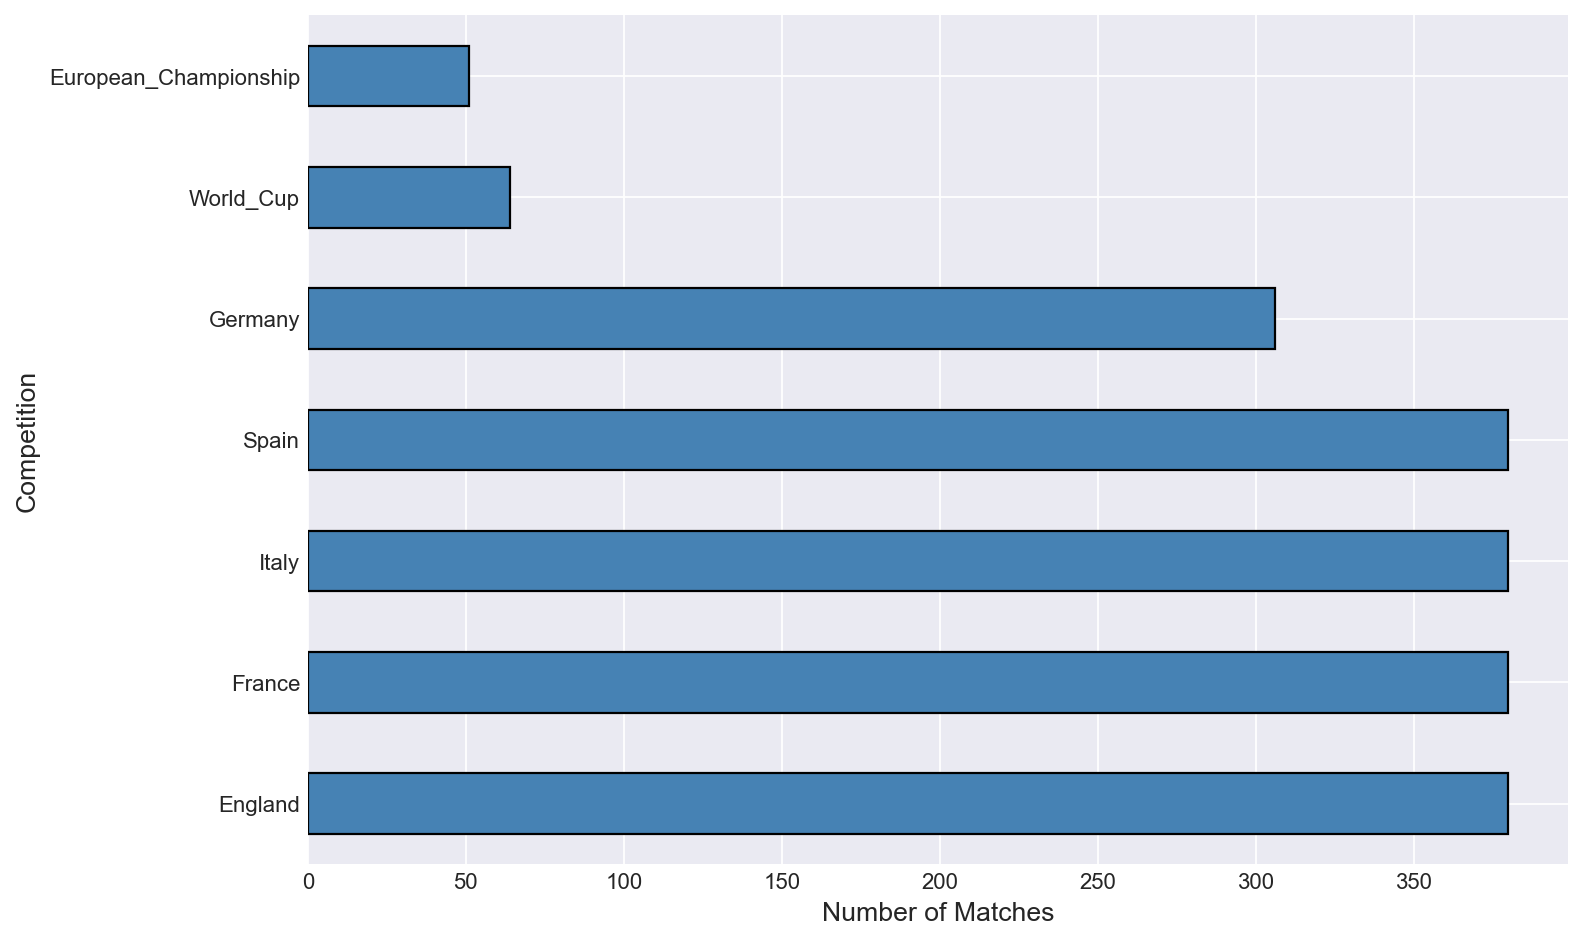
\includegraphics[width=0.85\linewidth]{figures/eda/matches_per_competition.png}
  \caption{Anzahl der Spiele pro Wettbewerb. Sowohl Liga-Wettbewerbe wie auch internationale Turniere}
  \label{fig:matches_per_competition}
\end{figure}

Der Datensatz umfasst mehrere europäische Top-Ligen sowie internationale Turniere. Abbildung~\ref{fig:matches_per_competition} zeigt die Verteilung der Spiele über die Wettbewerbe. Unterschiede in der Spielanzahl spiegeln Ligaformate (z.\,B. 38 Spieltage) und Turnierlängen wider.

Ergänzend zeigt Abbildung~\ref{fig:events_by_competition} die Anzahl der Ereignisse pro Wettbewerb. Erwartungsgemäss skaliert die Eventanzahl stark mit der Anzahl Spiele. Die Liga-Wettbewerbe (England, Spanien, Frankreich, Italien) weisen jeweils ca. 650{,}000 Events auf (ca. 1{,}710 Events pro Match), während Deutschland mit ca. 530{,}000 Events (ca. 1{,}730 Events/Match) und die Turniere World Cup und European Championship mit ca. 130{,}000 bzw. 100{,}000 Events eine geringere Gesamtzahl aufweisen. Dies bildet eine robuste Basis für detaillierte Netzwerkanalysen.

\begin{figure}[htbp]
  \centering
  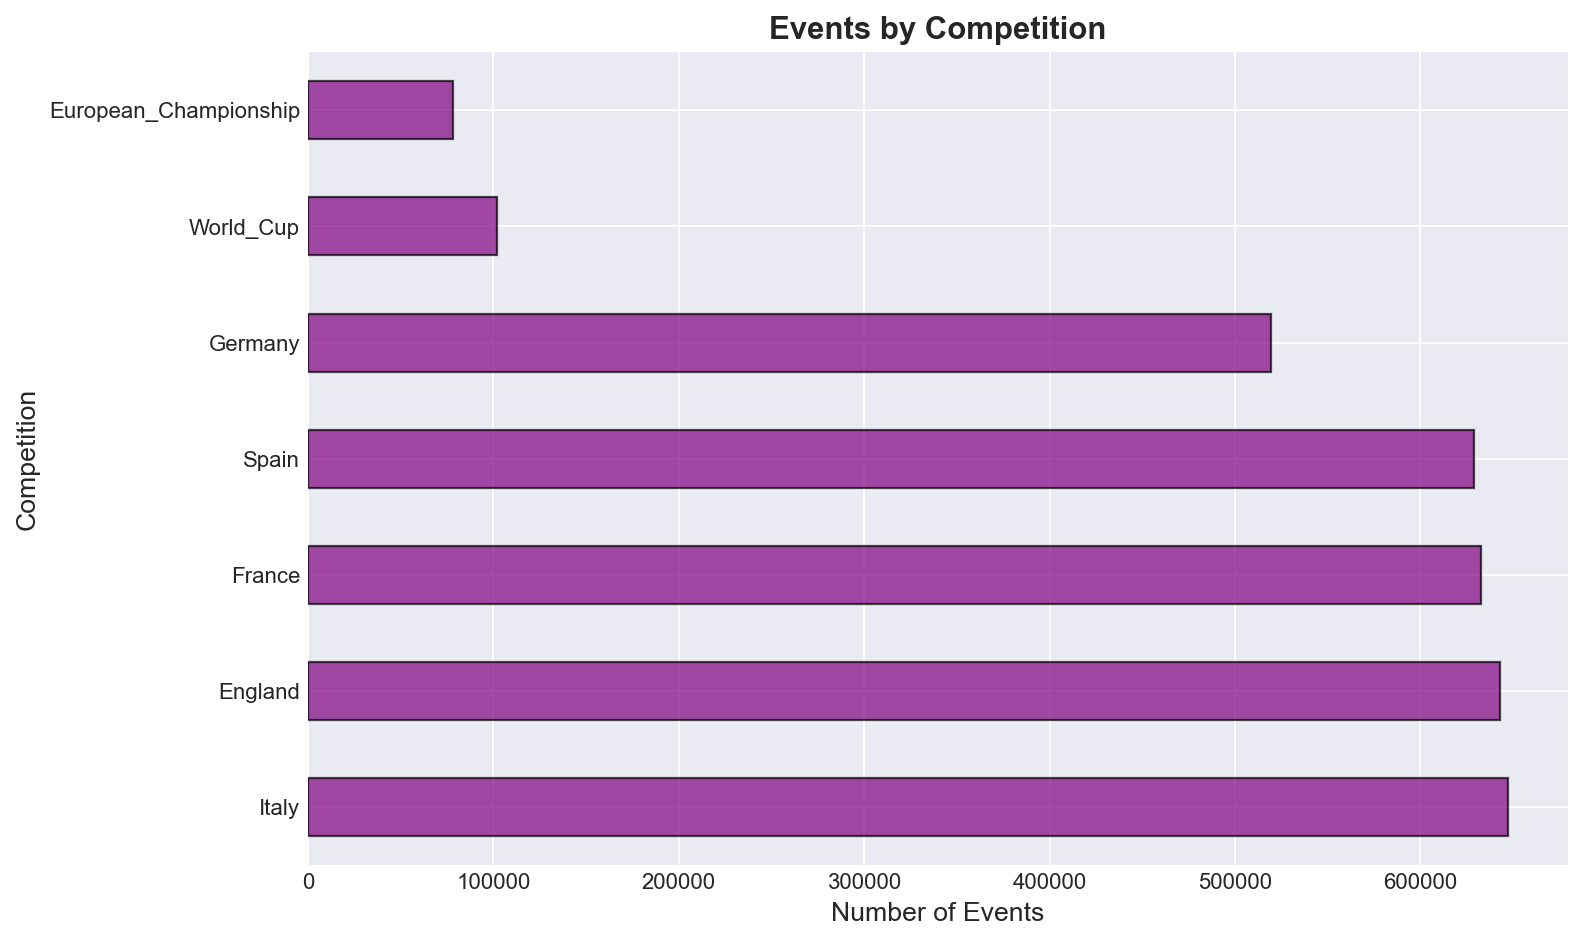
\includegraphics[width=0.85\linewidth]{figures/eda/events_by_competition.png}
  \caption{Anzahl der Events pro Wettbewerb. Stark abhängig vom Format des Turniers.}
  \label{fig:events_by_competition}
\end{figure}

Zur Veranschaulichung der Match-Metadaten zeigt Tabelle~\ref{tab:matches_sample} eine zufällige Stichprobe von 5 Spielen (\texttt{df.sample(5)} auf dem Match-DataFrame):

\begin{table}[htbp]
\centering
\small
\begin{tabularx}{\linewidth}{lllXXl}
\toprule
Team 1 & Team 2 & Score & Date & Venue & Duration \\
\midrule
Huddersfield Town & Crystal Palace & 0 - 2 & March 17, 2018 at 4:00:00 PM GMT+1 & The John Smith's Stadium & Regular \\ \addlinespace
Manchester United & Crystal Palace & 4 - 0 & Sept 30, 2017 at 4:00:00 PM GMT+2 & Old Trafford & Regular \\ \addlinespace
Everton & Southampton & 1 - 1 & May 5, 2018 at 6:30:00 PM GMT+2 & Goodison Park & Regular \\ \addlinespace
Everton & Manchester United & 0 - 2 & Jan 1, 2018 at 6:30:00 PM GMT+1 & Goodison Park & Regular \\ \addlinespace
Stoke City & Liverpool & 0 - 3 & Nov 29, 2017 at 9:00:00 PM GMT+1 & Bet365 Stadium & Regular \\
\bottomrule
\end{tabularx}
\caption{Beispiele von 5 zufällig ausgewählten Spielen aus dem Gesamtdatensatz mit Spielbezeichnung, Datum, Austragungsort und Spieldauer.}
\label{tab:matches_sample}
\end{table}

\subsection{Ereignisse: Typen und zeitliche Muster}

Die Event-Typen sind über IDs und Labels definiert; Tabelle~\ref{tab:event_types} dokumentiert diese Zuordnung und dient in späteren Kapiteln als Referenz für Filter und Aggregationen.

\begin{table}[htbp]
\centering
\small
\setlength{\tabcolsep}{3pt}
\begin{tabular}{lrrll}

\toprule
 & event & subevent & event\_label & subevent\_label \\
\midrule
0 & 1 & 10 & Duel & Air duel \\
1 & 1 & 11 & Duel & Ground attacking duel \\
2 & 1 & 12 & Duel & Ground defending duel \\
3 & 1 & 13 & Duel & Ground loose ball duel \\
4 & 2 & 20 & Foul & Foul \\
5 & 2 & 21 & Foul & Hand foul \\
6 & 2 & 22 & Foul & Late card foul \\
7 & 2 & 23 & Foul & Out of game foul \\
8 & 2 & 24 & Foul & Protest \\
9 & 2 & 25 & Foul & Simulation \\
10 & 2 & 26 & Foul & Time lost foul \\
11 & 2 & 27 & Foul & Violent Foul \\
12 & 3 & 30 & Free Kick & Corner \\
13 & 3 & 31 & Free Kick & Free Kick \\
14 & 3 & 32 & Free Kick & Free kick cross \\
15 & 3 & 33 & Free Kick & Free kick shot \\
16 & 3 & 34 & Free Kick & Goal kick \\
17 & 3 & 35 & Free Kick & Penalty \\
18 & 3 & 36 & Free Kick & Throw in \\
19 & 4 & 40 & Goalkeeper leaving line & Goalkeeper leaving line \\
20 & 5 & 50 & Interruption & Ball out of the field \\
21 & 5 & 51 & Interruption & Whistle \\
22 & 6 & 60 & Offside & Offside \\
23 & 7 & 70 & Others on the ball & Acceleration \\
24 & 7 & 71 & Others on the ball & Clearance \\
25 & 7 & 72 & Others on the ball & Touch \\
26 & 8 & 80 & Pass & Cross \\
27 & 8 & 81 & Pass & Hand pass \\
28 & 8 & 82 & Pass & Head pass \\
29 & 8 & 83 & Pass & High pass \\
30 & 8 & 84 & Pass & Launch \\
31 & 8 & 85 & Pass & Simple pass \\
32 & 8 & 86 & Pass & Smart pass \\
33 & 9 & 90 & Save attempt & Reflexes \\
34 & 9 & 91 & Save attempt & Save attempt \\
35 & 10 & 100 & Shot & Shot \\
\bottomrule
\end{tabular}
\caption{Vollständige Übersicht der Ereignistypen und Subtypen im Datensatz. Die Spalten geben die Event-ID und Subevent-ID sowie deren sprachliche Bezeichnung an.}
\label{tab:event_types}
\end{table}

Die Analyse der Ereignistypen in Abbildung~\ref{fig:event_types_top15} zeigt erwartungsgemäss, dass Pässe die häufigste Aktion darstellen, gefolgt von Duellen und Ballkontakten. Diese Dominanz von Passereignissen motiviert den den Schwerpunkt in der analyse später auf ein Passnetzwerke zu legen.

\begin{figure}[htbp]
  \centering
  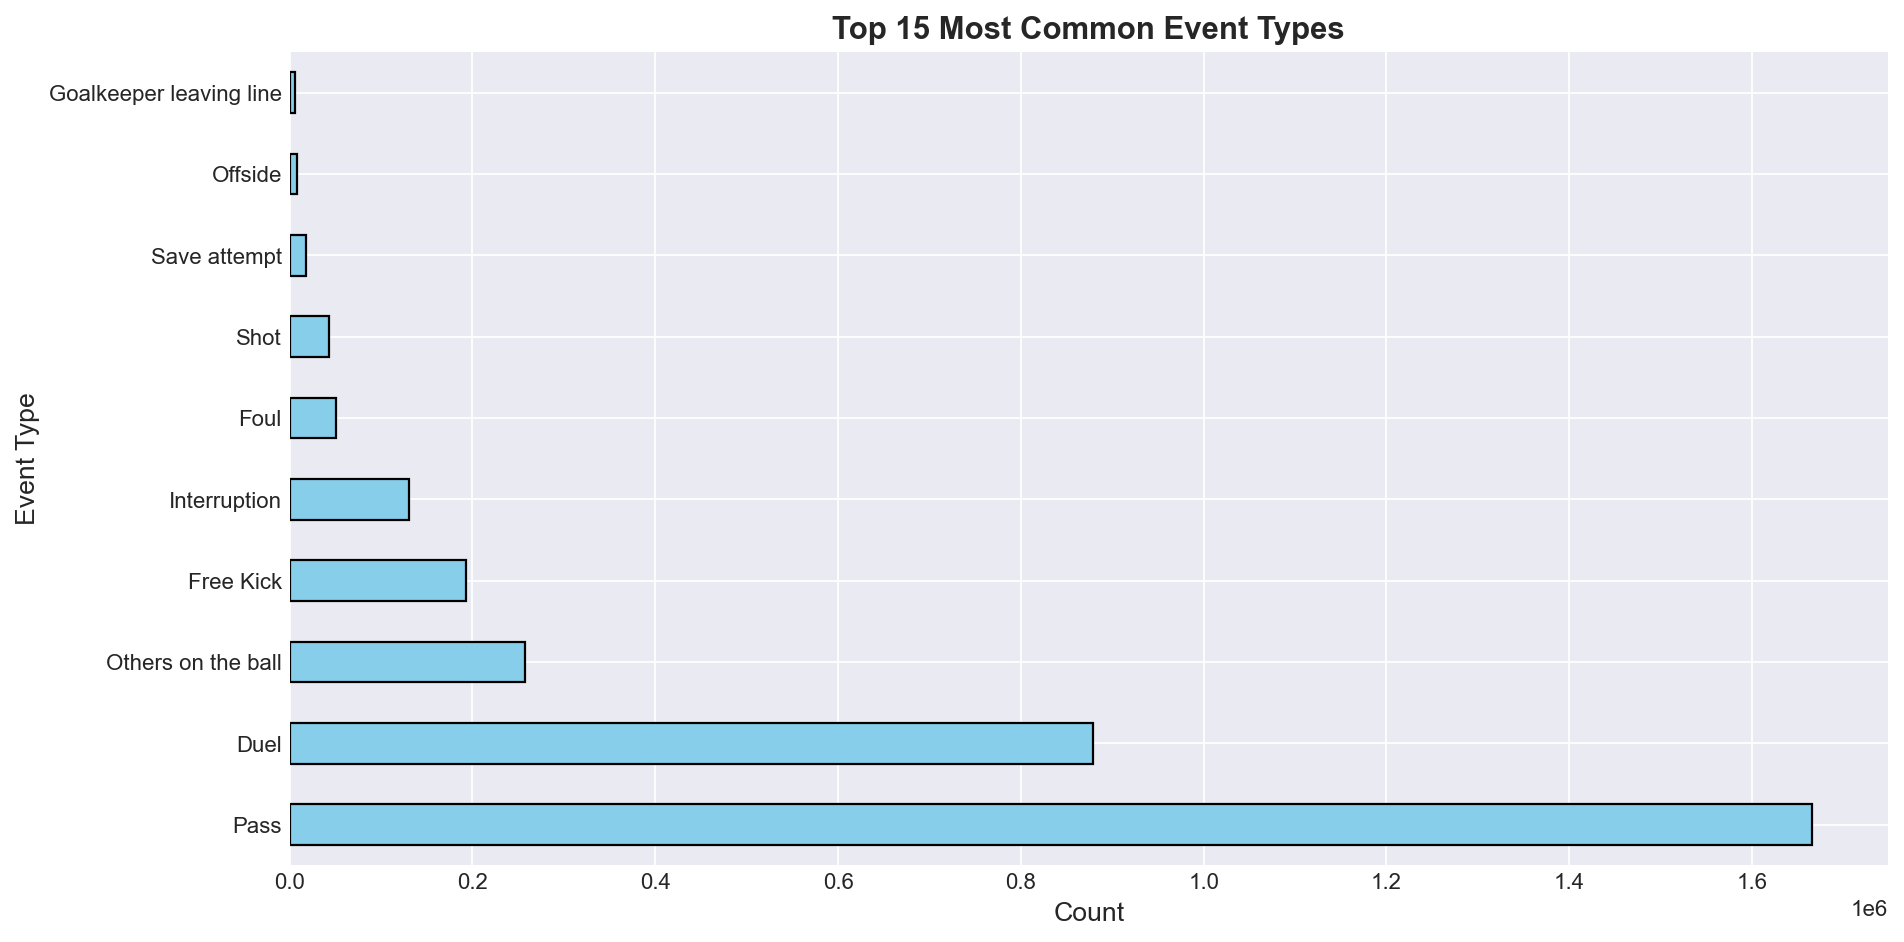
\includegraphics[width=0.9\linewidth]{figures/eda/event_types_top15.png}
  \caption{Top 15 Ereignistypen über alle Wettbewerbe. Pässe dominieren klar das Spielgeschehen.}
  \label{fig:event_types_top15}
\end{figure}

Die zeitliche Verteilung der Ereignisse über den Spielverlauf (Abbildung~\ref{fig:events_per_minute}) zeigt erhöhte Aktivität zu Beginn beider Halbzeiten sowie einen Abfall gegen Ende der Halbzeiten.

\begin{figure}[htbp]
  \centering
  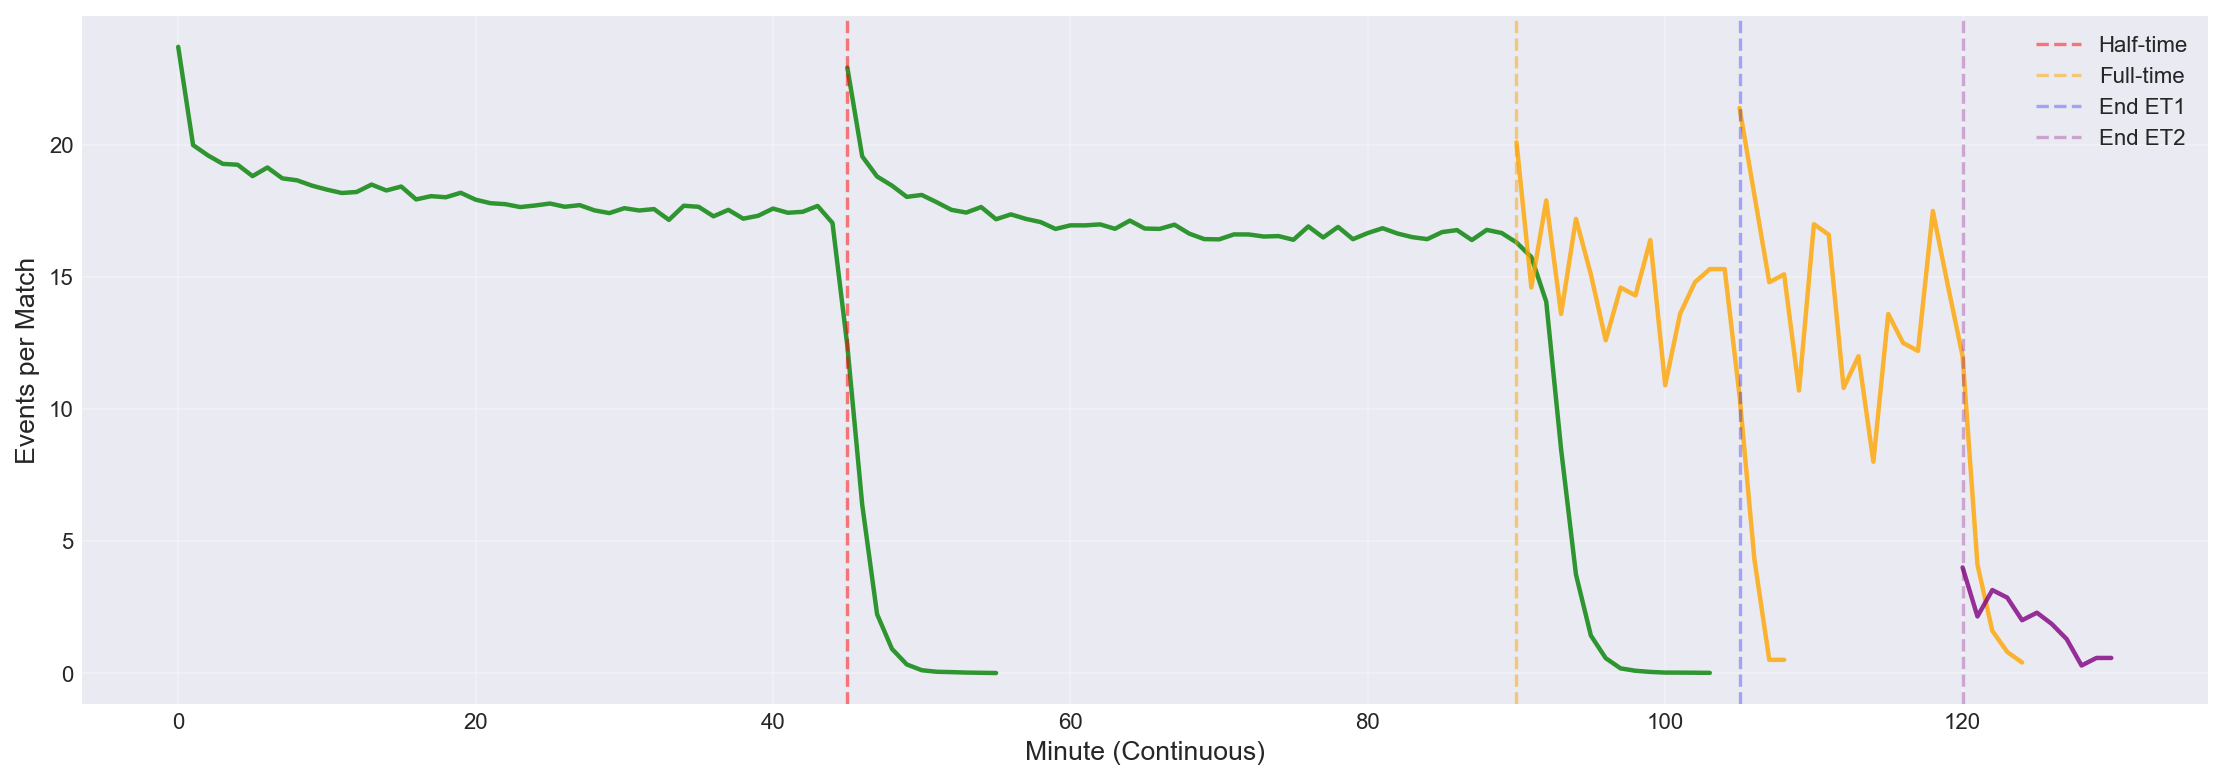
\includegraphics[width=0.9\linewidth]{figures/eda/events_per_minute_normalized.png}
  \caption{Ereignisse pro Spielminute. Deutlich erkennbar sind erhöhte Aktivität zu Spielbeginn und der Rückgang in der Schlussphase.}
  \label{fig:events_per_minute}
\end{figure}

Auf aggregierter Ebene ist die Datenabdeckung über die reguläre Spielzeit ausgeglichen: Abbildung~\ref{fig:events_by_period} zeigt nahezu identische Event-Zahlen in der ersten und zweiten Halbzeit (je ca. \num{1.62e6} Events).

\begin{figure}[htbp]
  \centering
  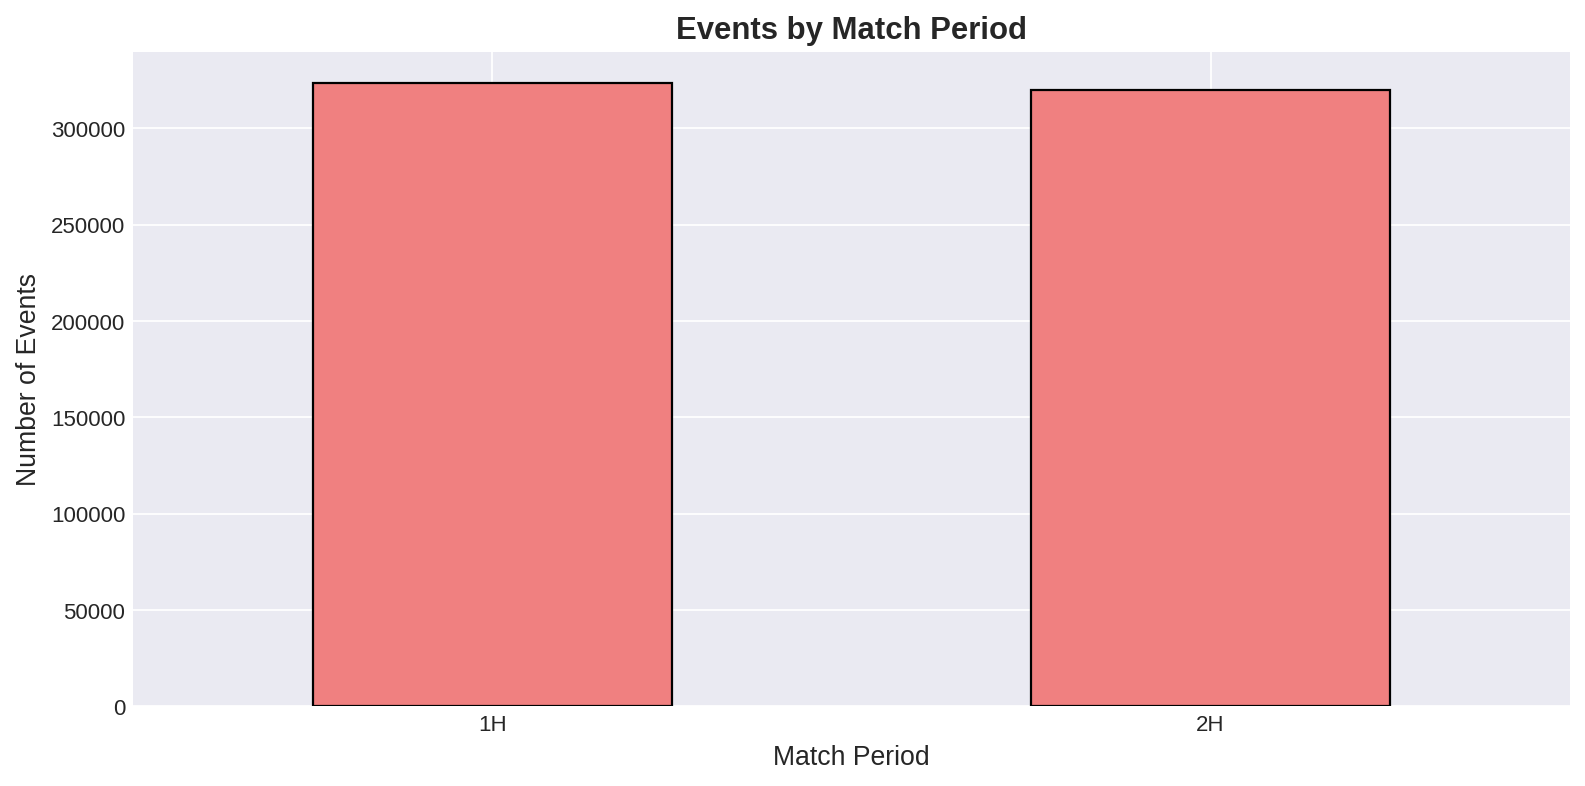
\includegraphics[width=0.7\linewidth]{figures/eda/events_by_period.png}
  \caption{Events nach Spielperiode. In der vorliegenden Auswertung sind beide \textbf{H}albzeiten mit je über \num{1.62e6} Events nahezu gleich stark vertreten. \textbf{E}xtended 1 / 2 sowie \textbf{P}enaly kommen bedeutend seltener vor (10 / 10 / 7)}
  \label{fig:events_by_period}
\end{figure}

Für Passereignisse zeigt sich jedoch ein leichter Halbzeiteffekt (Abbildung~\ref{fig:passes_by_period}): In der ersten Halbzeit werden mehr Pässe gespielt, die Passgenauigkeit ist minimal höher (82.99\% vs. 82.06\%) und die durchschnittliche Passdistanz praktisch unverändert (24.69 vs. 24.54). Dies passt zu Effekten wie Ermüdung, Spielstandmanagement oder erhöhtem Druck in Halbzeit 2.

\begin{figure}[htbp]
  \centering
  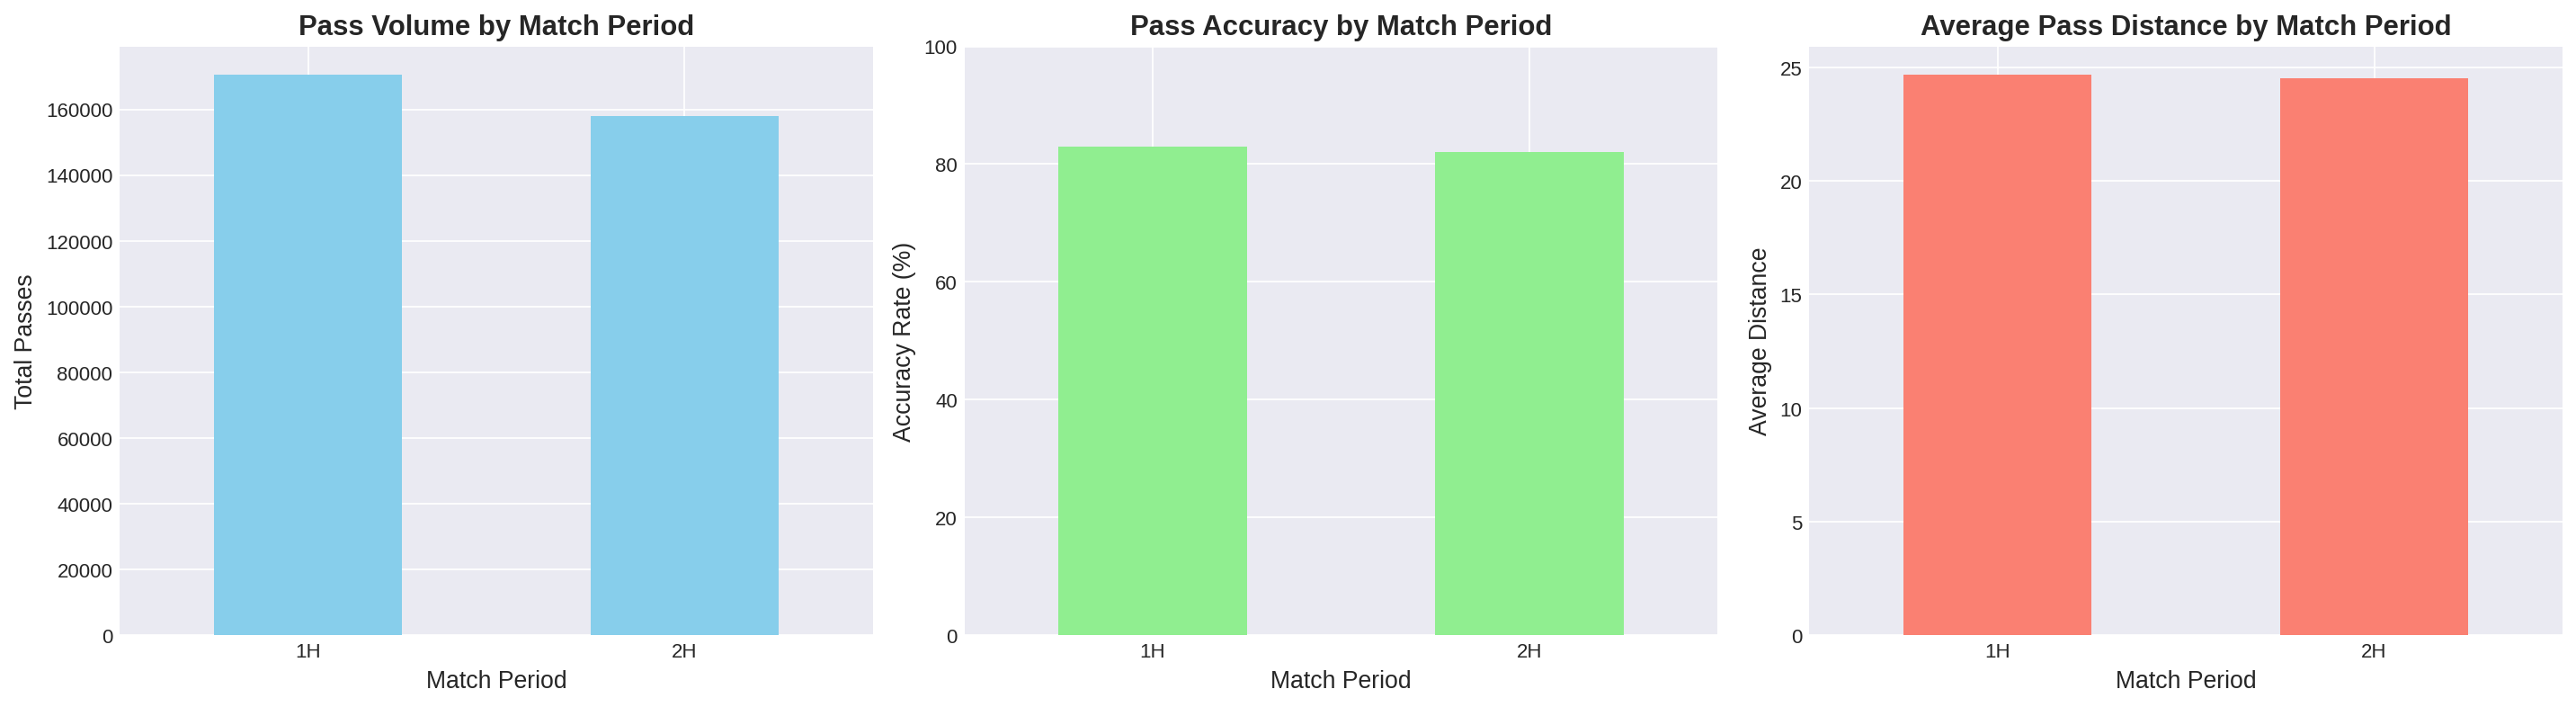
\includegraphics[width=\linewidth]{figures/eda/passes_by_period.png}
  \caption{Passvolumen, Passgenauigkeit und durchschnittliche Passdistanz nach Matchperiode. In dieser Auswertung werden in Halbzeit 1 mehr Pässe gespielt (+7.4\%), bei sehr ähnlicher Genauigkeit und Distanz.}
  \label{fig:passes_by_period}
\end{figure}

Während der Verlängerungsphasen ist eine Zunahme der Passlänge bei gleichzeitig abnehmender Genauigkeit zu verzeichnen. Diese Verhaltensweise lässt sich durch eine aggressivere Spielweise erklären, mit der versucht wird, ein Penalty-Szenario zu vermeiden. Ausserdem wird mit diesen Pässen hauptsächlich das Ziel verfolgt, Fehler zu vermeiden, indem eine möglichst grosse Distanz zum eigenen Tor geschaffen wird (A. Scheifele, persönliche Kommunikation, 30. Dezember 2025).

\subsection{Pass-Analyse: Zentrale Akteure und räumliche Verteilung}

Pässe bilden neben Teams \& Spielen das Rückgrat der späteren Netzwerkanalyse. Abbildung~\ref{fig:top_passers} identifiziert die aktivsten Passgeber. Diese Spieler sind Kandidaten für zentrale Knoten (hohe Degree- und Betweennesszentralität), da sie als Verteiler im Spielaufbau fungieren.

\begin{figure}[htbp]
  \centering
  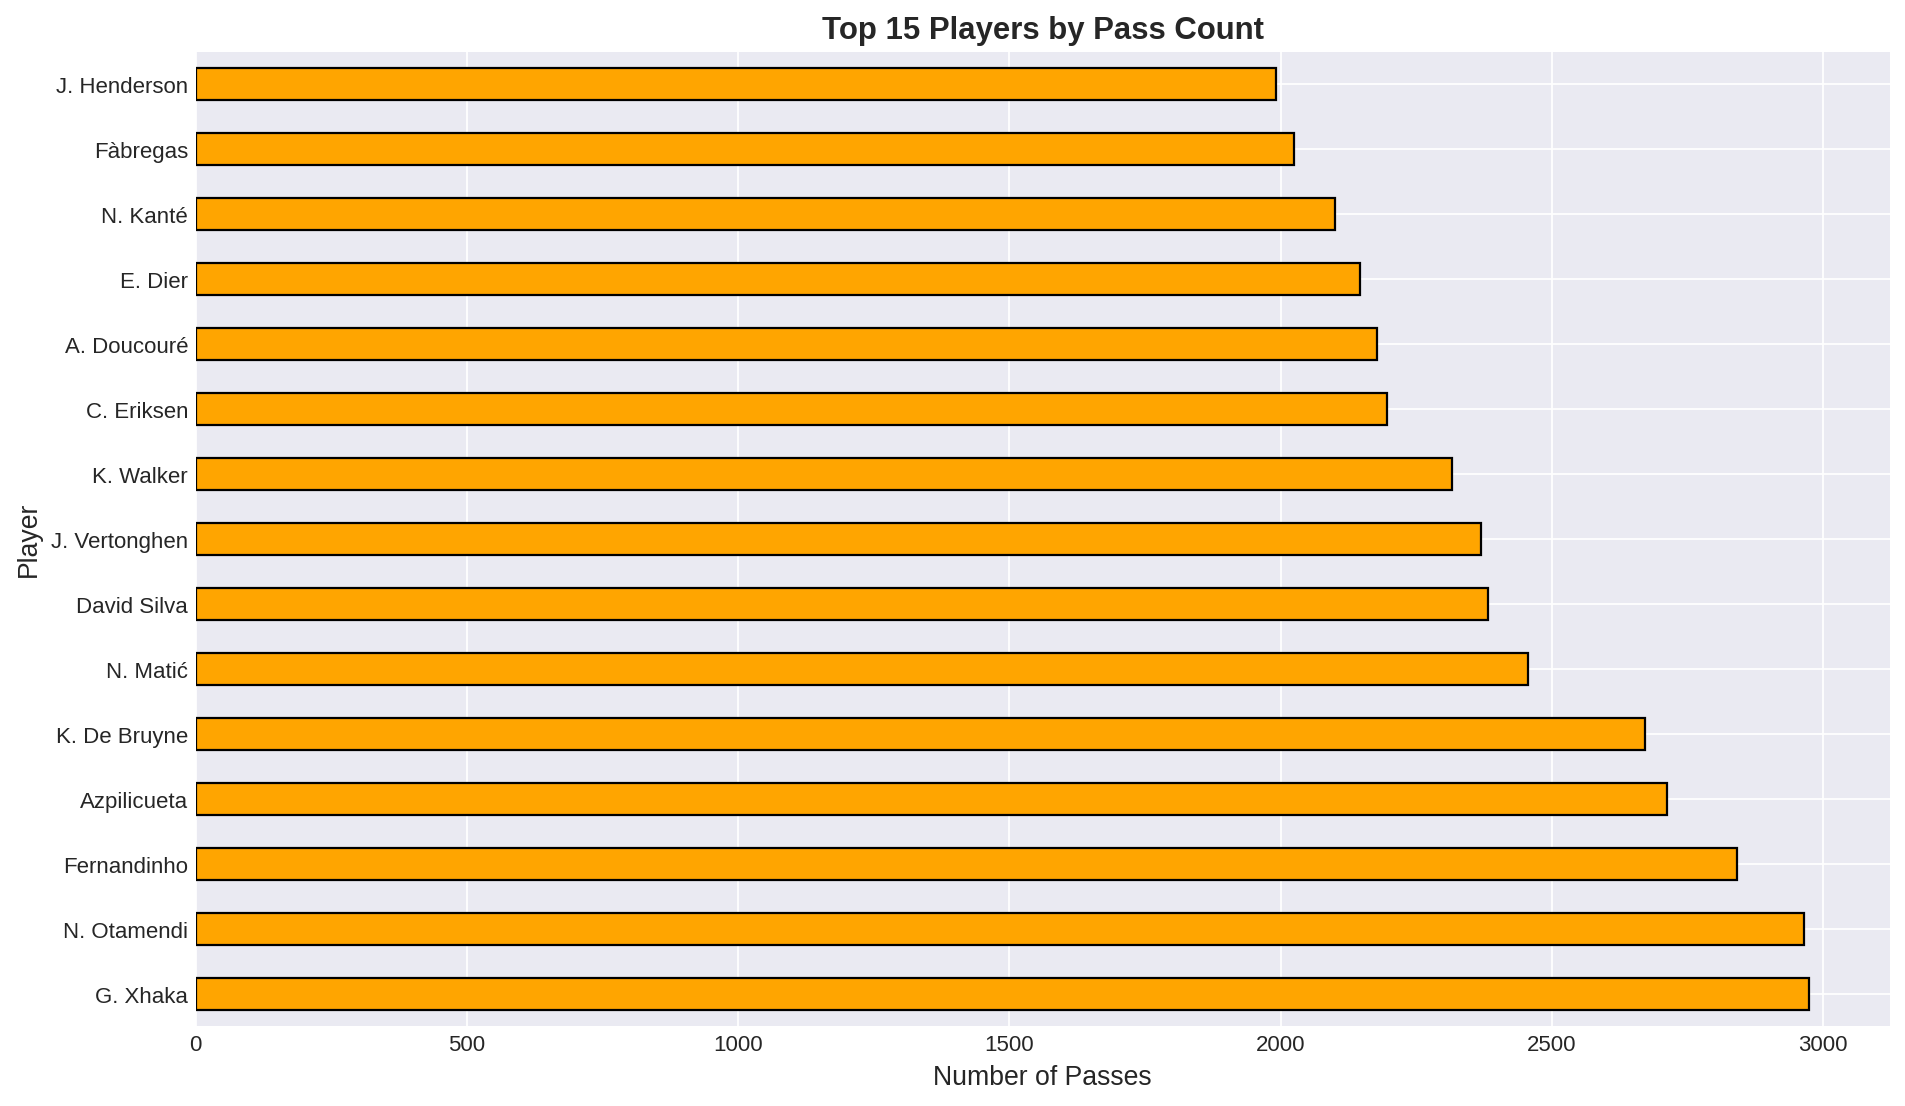
\includegraphics[width=0.85\linewidth]{figures/eda/top_passers.png}
  \caption{Top 15 Spieler nach Anzahl der Pässe. Diese Spieler sind später als zentrale Knoten in den Passnetzwerken zu erwarten.}
  \label{fig:top_passers}
\end{figure}

\begin{figure}[htbp]
  \centering
  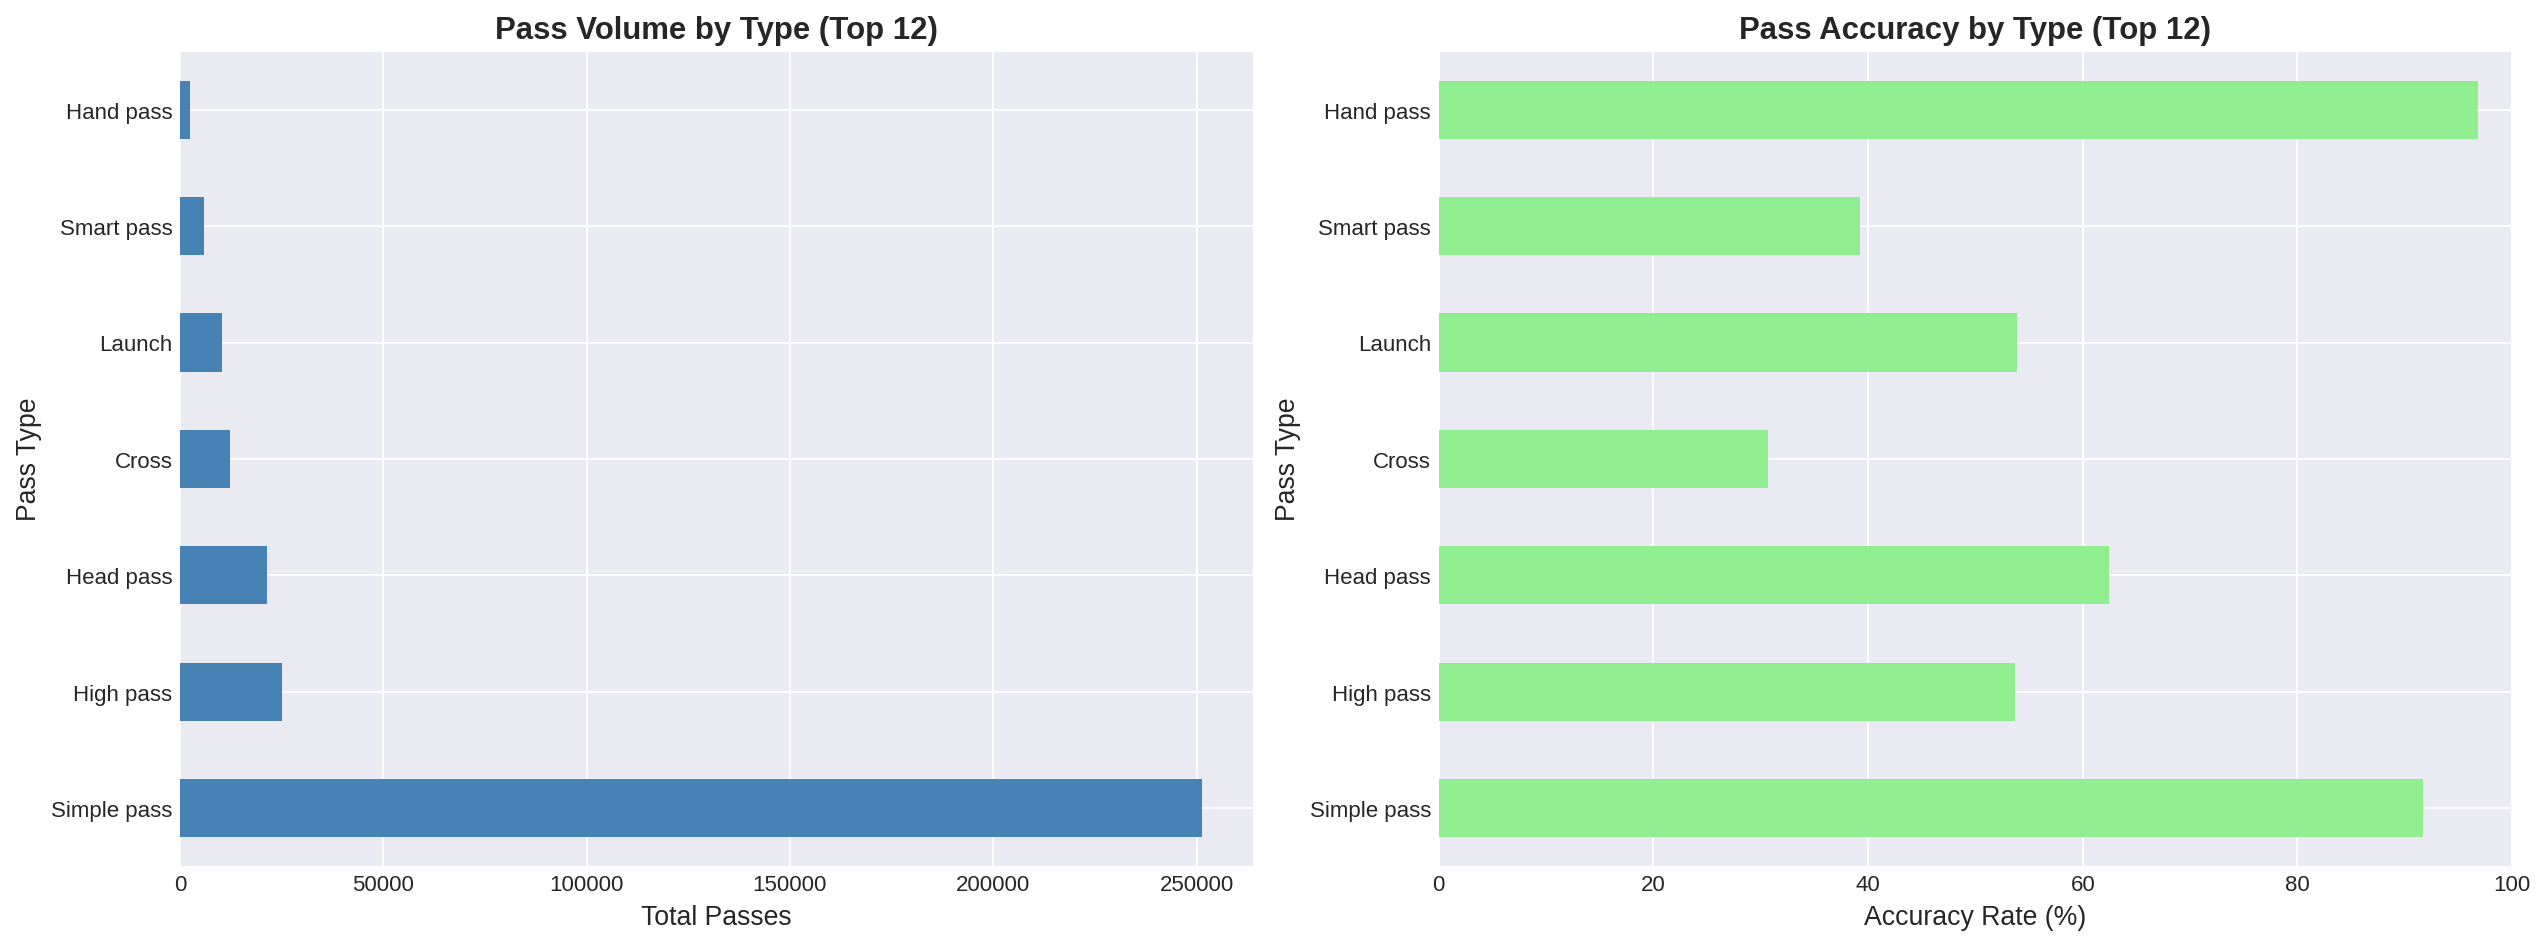
\includegraphics[width=\linewidth]{figures/eda/pass_types_analysis.png}
  \caption{Passvolumen (links) und Passgenauigkeit (rechts) nach Passtyp. Einfache Pässe dominieren das Volumen bei hoher Genauigkeit; Flanken und Smart Passes sind seltener und deutlich ungenauer. Handpässe verzeichnen aufgrund der manuellen Ballkontrolle und ihrer exklusiven Anwendung durch den Torhüter die höchste Präzision.}
  \label{fig:pass_types_analysis}
\end{figure}

Sowohl räumlichen Mustern als auch die Struktur nach Passtyp sind zentral für die Interpretation von Netzwerkkanten: Abbildung~\ref{fig:pass_types_analysis} zeigt, dass einfache Pässe den Grossteil des Volumens ausmachen (ca. 76\% aller Pässe) und zugleich eine sehr hohe Genauigkeit aufweisen (> 91\%). Risikoreichere Pässe (Flanken, Smart Passes) treten seltener auf und haben deutlich niedrigere Erfolgsraten (z.\,B. Flanken ca. 30.71\%). Für die spätere Netzwerkanalyse von Passlängen bedeutet dies: Gewichte werden stark durch kurze, sichere Verbindungen dominiert, während wenige riskante Kanten eher spielentscheidende Situationen abbilden.

Eine detaillierte räumliche Analyse der Pässe (Abbildung~\ref{fig:pass_distance_analysis}) liefert mehrere wichtige Erkenntnisse:
\begin{itemize}
  \item Die \textbf{Passlängenverteilung} (oben links) zeigt eine rechtssteile Verteilung mit Median bei ca. 15 Einheiten, was kurzen bis mittellangen Pässen entspricht. Lange Bälle sind seltener.
  \item Die \textbf{Passlängen nach Typ} (oben rechts) verdeutlichen erwartbare Unterschiede: Lange Bälle und Flanken weisen deutlich grössere Distanzen auf als einfache Zuspiele.
  \item Die \textbf{Heatmaps} (unten) für Pass-Ursprung und -Ziel zeigen die räumliche Konzentration: Viele Pässe starten und enden im Mittelfeld sowie in defensiven Bereichen, während Pässe im gegnerischen Strafraum seltener sind.
\end{itemize}

\begin{figure}[htbp]
  \centering
  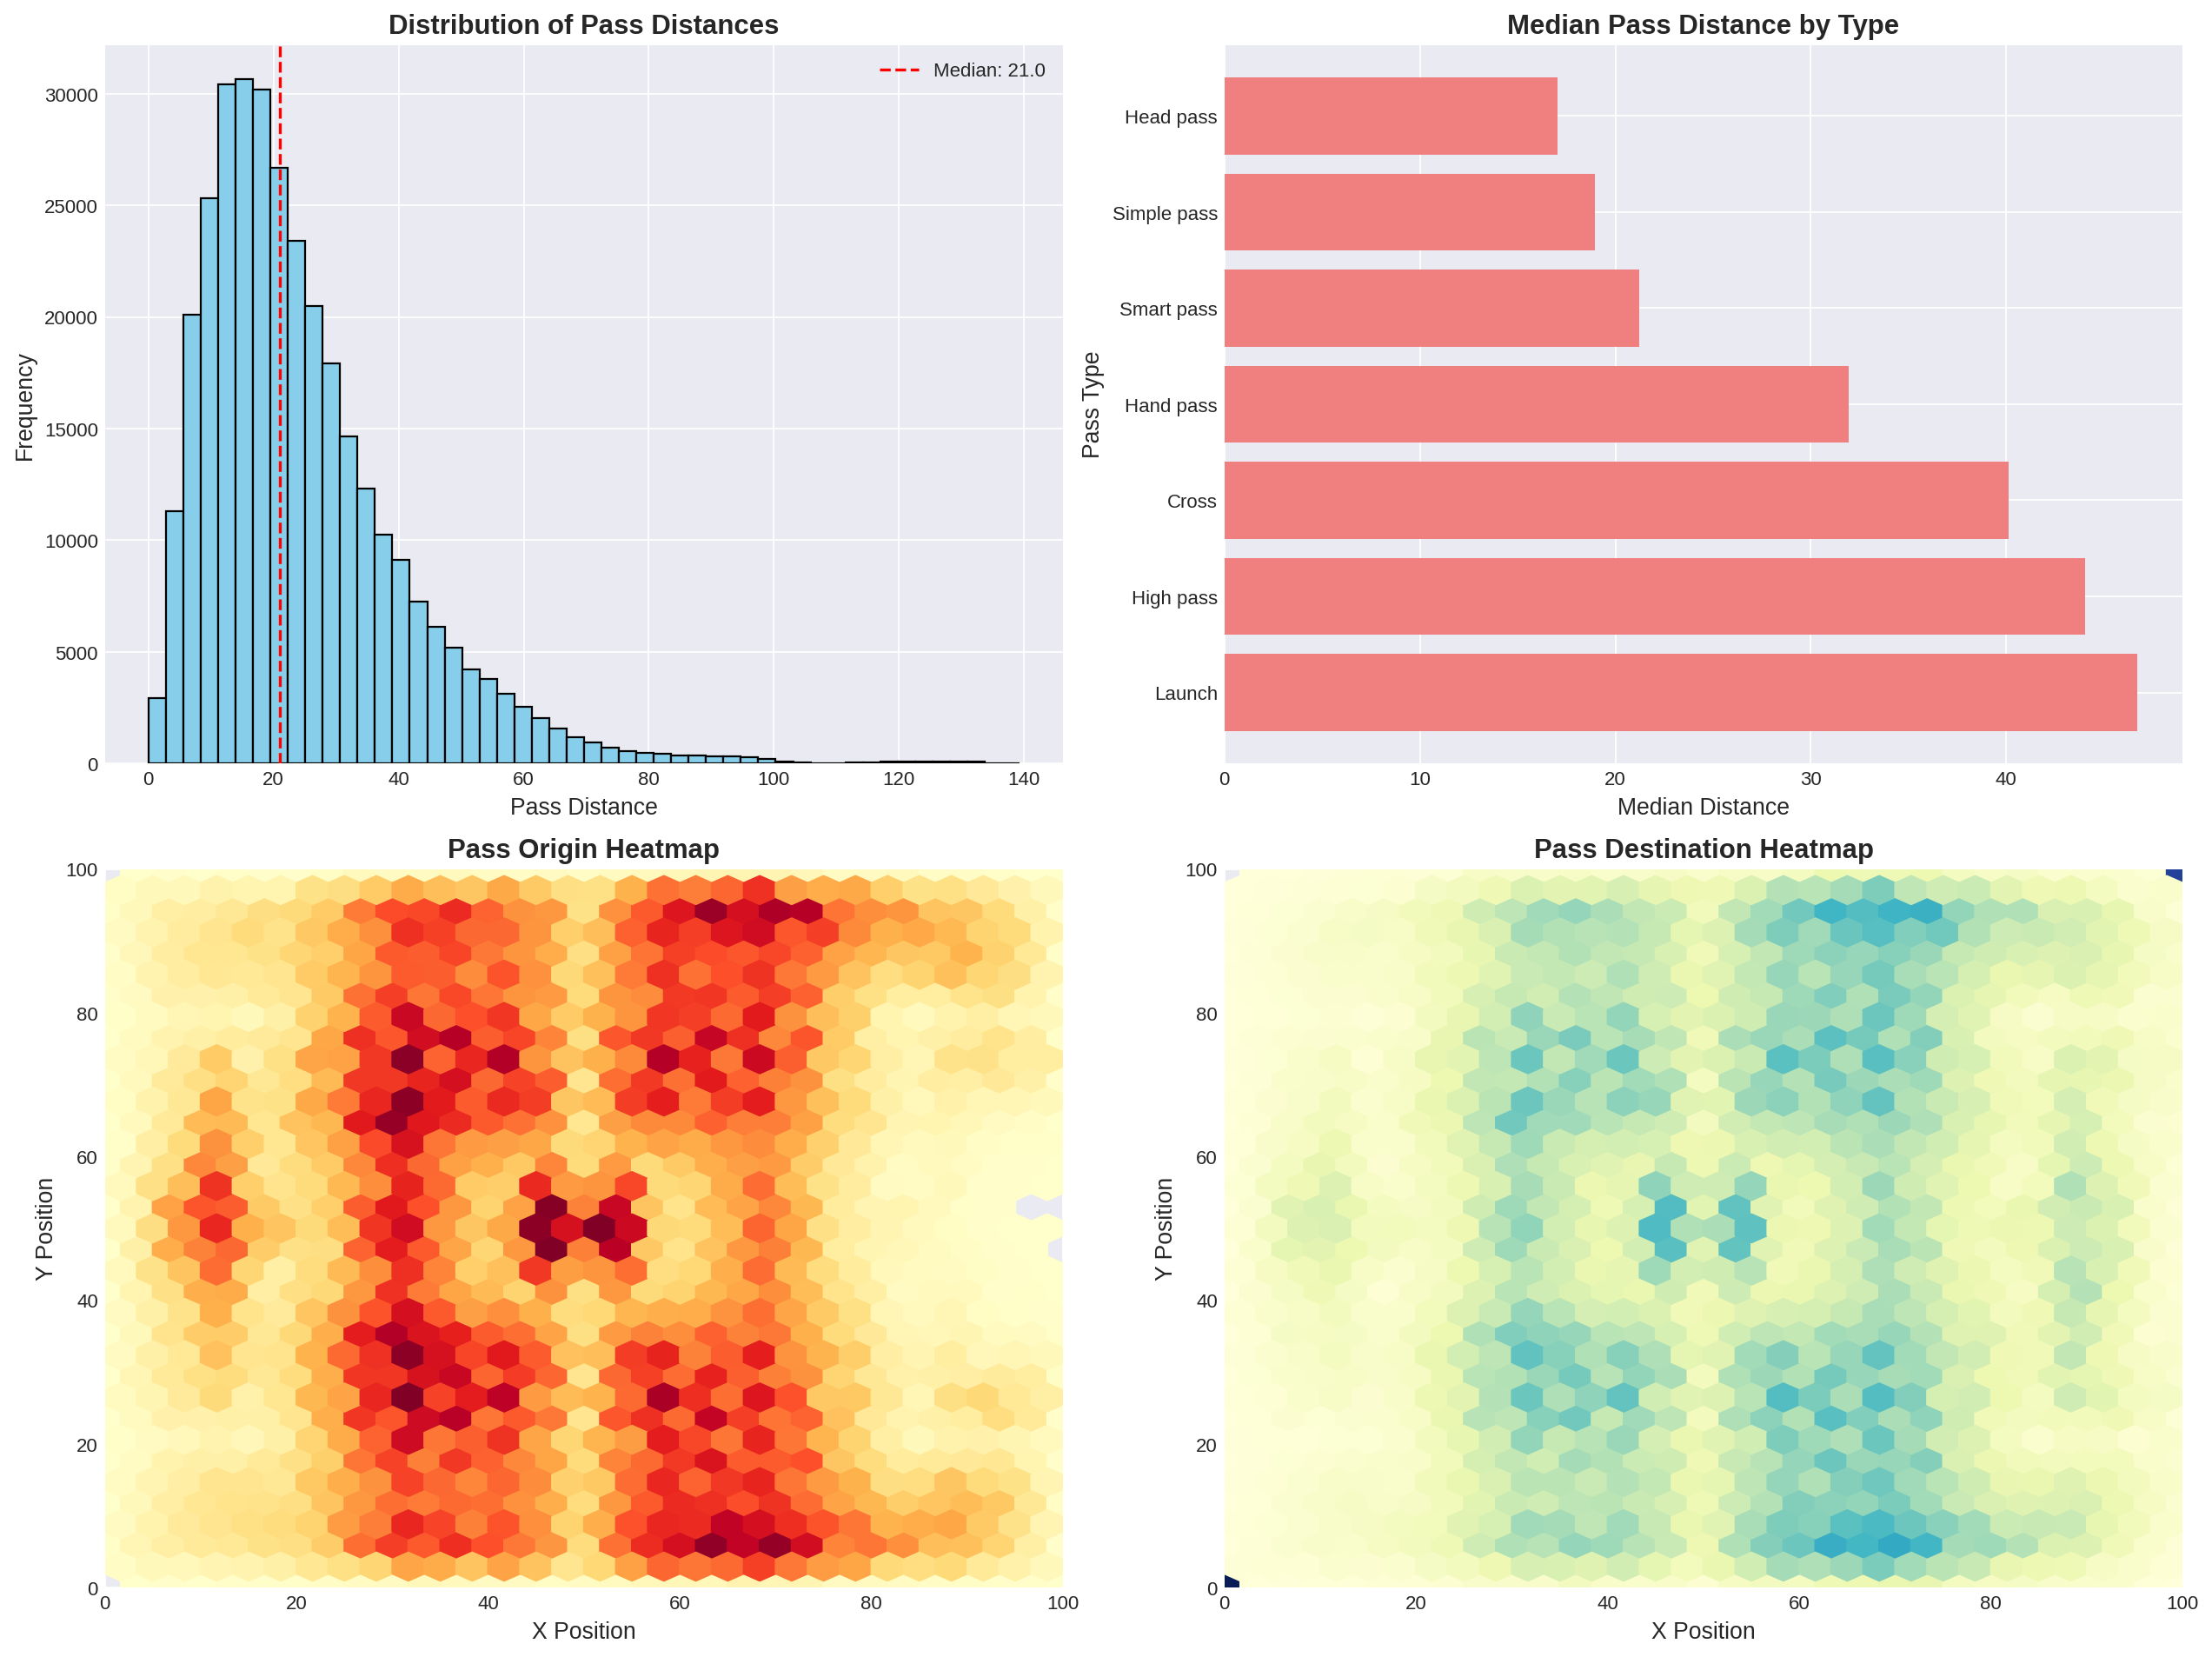
\includegraphics[width=\linewidth]{figures/eda/pass_distance_analysis.png}
  \caption{Umfassende Analyse der Passeigenschaften. \textbf{Oben links:} Verteilung der Passlängen mit Median-Markierung. \textbf{Oben rechts:} Median-Passlänge nach Passtyp (z.\,B. lange Bälle vs. kurze Zuspiels). \textbf{Unten:} Heatmaps für Pass-Ursprung (links) und Pass-Ziel (rechts), visualisiert auf normalisierten Spielfeldkoordinaten.}
  \label{fig:pass_distance_analysis}
\end{figure}

Abbildung~\ref{fig:network_metrics_sample} illustriert die Rolleninterpretation einfacher Zentralitätskonzepte (Degreezentralität in diesem Fall) in einem Beispielspiel: Spieler oberhalb der Diagonalen erhalten mehr Pässe als sie spielen (Zielspieler), Spieler unterhalb verteilen mehr (Aufbauspieler), und Spieler nahe der Diagonalen sind ausgeglichen. Generell können wir erkennen: wer mehr Pässe bekommt, vergibt auch mehr.

\begin{figure}[htbp]
  \centering
  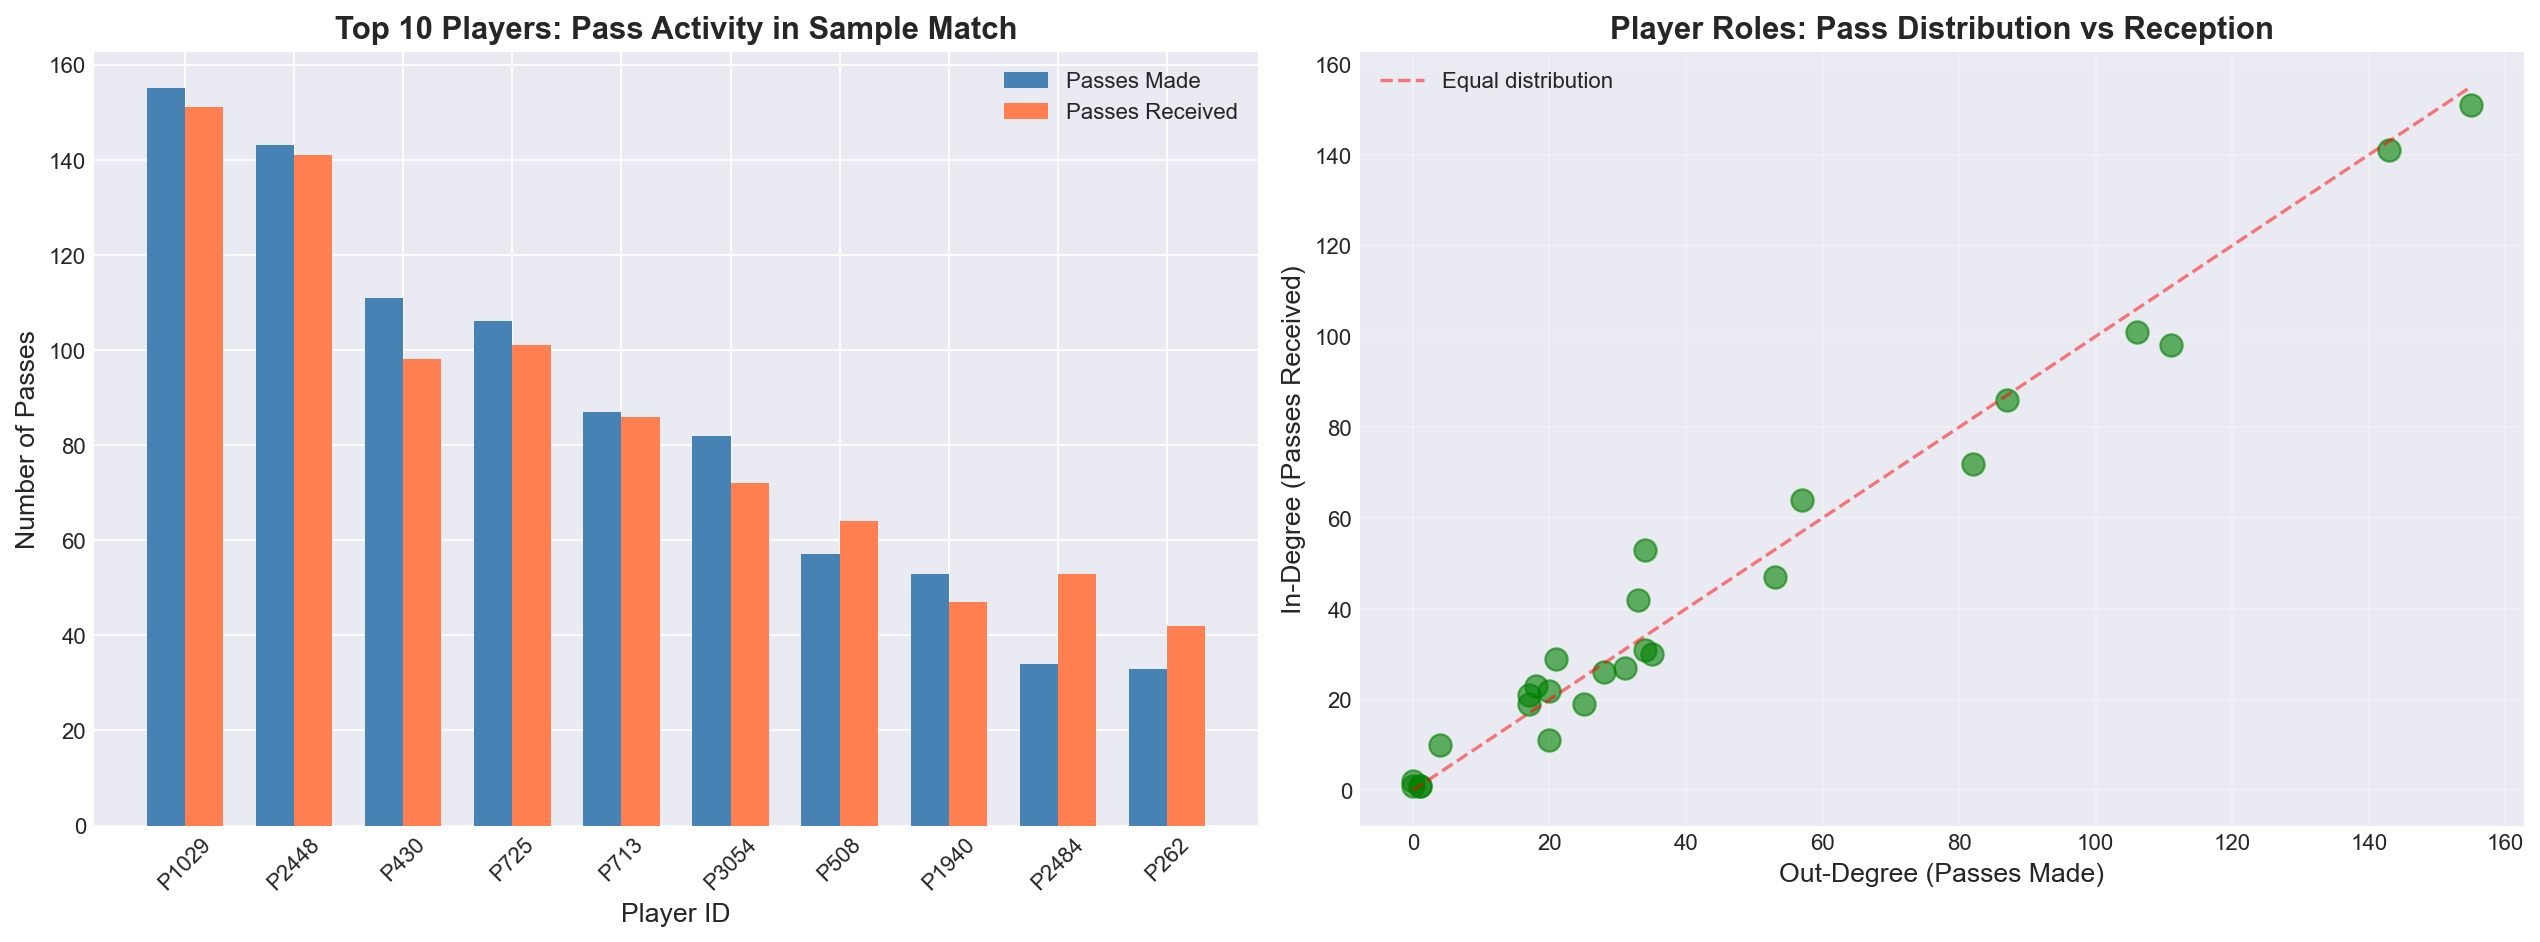
\includegraphics[width=\linewidth]{figures/eda/network_metrics_sample.png}
  \caption{Passverhältniss in einem Sample-Match: (links) Top-10 Spieler nach Passvolumen (gespielt vs. empfangen), (rechts) Out-Degree vs. In-Degree mit Referenzlinie $y=x$ zur Rolleninterpretation.}
  \label{fig:network_metrics_sample}
\end{figure}

Um die spätere Netzwerkkonstruktion zu illustrieren, zeigt Tabelle~\ref{tab:pass_network_sample} einen Ausschnitt aus einem berechneten Passnetzwerk eines Beispielspiels (Match-ID 2500004). Die Kanten sind Passverbindungen, gewichtet nach \textit{pass\_count}; zusätzlich ist die mittlere Passdistanz angegeben.

\begin{table}[htbp]
\centering
\small
\setlength{\tabcolsep}{4pt}
\begin{tabular}{lrrrrll}
\toprule
 & passer\_id & receiver\_id & pass\_count & avg\_distance & passer\_name & receiver\_name \\
\midrule
0 & 3324 & 8625.000000 & 1 & 4.123106 & Álvaro Morata & V. Moses \\
1 & 3350 & 3324.000000 & 1 & 13.038405 & Fàbregas & Álvaro Morata \\
2 & 3350 & 3360.000000 & 6 & 20.523277 & Fàbregas & Pedro \\
3 & 3350 & 3429.000000 & 3 & 25.654240 & Fàbregas & T. Courtois \\
4 & 3350 & 8032.000000 & 1 & 26.627054 & Fàbregas & Marcos Alonso \\
5 & 3350 & 8495.000000 & 3 & 12.648930 & Fàbregas & D. Drinkwater \\
6 & 3350 & 8625.000000 & 2 & 21.530491 & Fàbregas & V. Moses \\
7 & 3350 & 14748.000000 & 3 & 9.815600 & Fàbregas & A. Rüdiger \\
8 & 3350 & 25553.000000 & 9 & 18.920233 & Fàbregas & Azpilicueta \\
9 & 3350 & 25707.000000 & 1 & 17.804494 & Fàbregas & E. Hazard \\
\bottomrule
\end{tabular}
\caption{Ausschnitt eines Passnetzwerks: erste 10 Passverbindungen eines Beispielspiels (Match-ID 2500004) mit Anzahl der Pässe, mittlerer Distanz und Spielernamen.}
\label{tab:pass_network_sample}
\end{table}

\subsection{Wettbewerbsvergleich}

Die aggregierten Pass-Statistiken nach Wettbewerb (Abbildung~\ref{fig:competition_pass_stats}) ermöglichen einen direkten Vergleich der Spielstile: Volumen (Anzahl der Pässe), Genauigkeit (Erfolgsquote) und durchschnittliche Passlänge variieren zwischen den Ligen und Turnieren. Solche Unterschiede können auf taktische Präferenzen, Spieltempo oder die Qualität der Teams hindeuten und werden sich in den strukturellen Eigenschaften der daraus generierten Netzwerke widerspiegeln.

\begin{figure}[htbp]
  \centering
  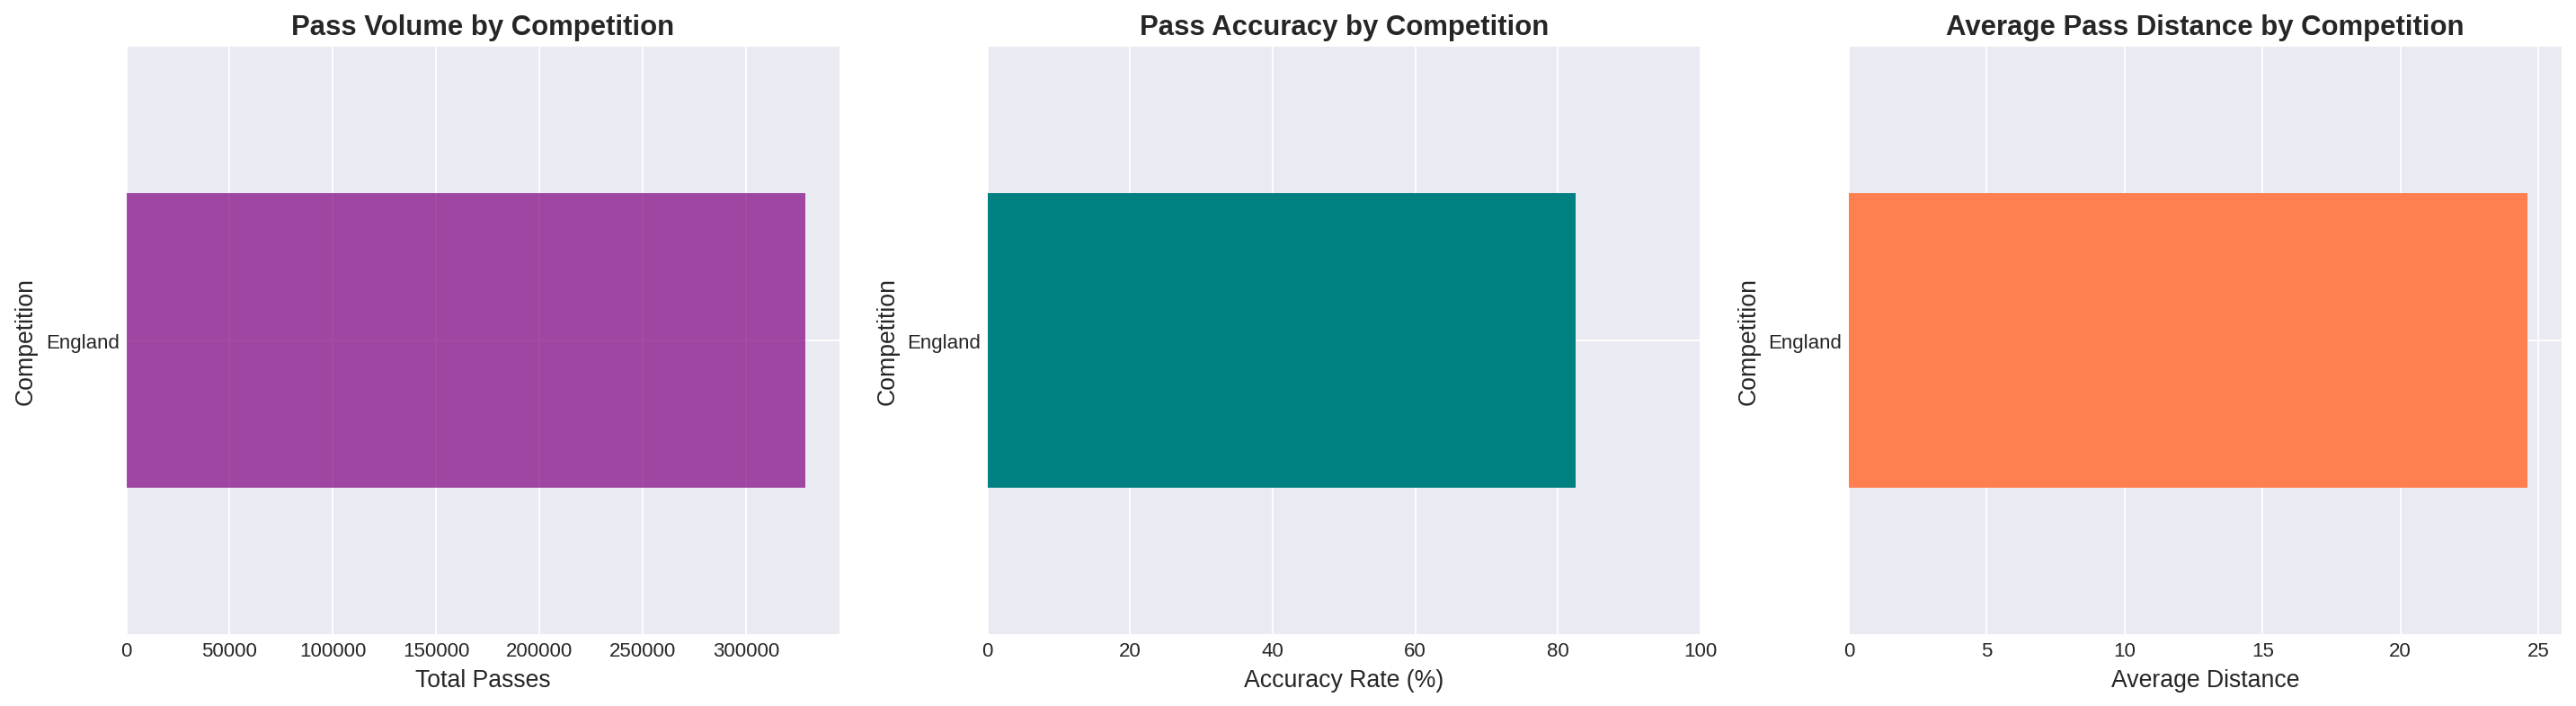
\includegraphics[width=\linewidth]{figures/eda/competition_pass_stats.png}
  \caption{Pass-Statistiken nach Wettbewerb: Volumen, Genauigkeit und durchschnittliche Distanz. Unterschiede deuten auf verschiedene Spielstile und taktische Ansätze hin.}
  \label{fig:competition_pass_stats}
\end{figure}

Auf Basis der vorliegenden Wettbewerbsauswertung liegt die Passgenauigkeit der englischen Liga bei ca. 82.5\% (Abbildung~\ref{fig:competition_pass_stats}), was im professionellen Fussball ein typischer Wert ist (etwa 4 von 5 Pässen kommen an) \parencite{fotmob_no_date}.

\subsection{Erste Hypothesen für die Netzwerk-Analyse}

Basierend auf den EDA-Ergebnissen lassen sich folgende Hypothesen für die nachfolgenden Netzwerkanalysen:

\begin{enumerate}
  \item \textbf{Zentrale Knoten:} Die identifizierten Top-Passgeber werden hohe Degree-Zentralität und Betweenness-Zentralität aufweisen, da sie als Verteiler im Spielaufbau fungieren.
  \item \textbf{Räumliche Cluster:} Die Heatmaps deuten auf räumliche Cluster hin (Abwehr, Mittelfeld, Angriff), die sich in Communitystrukturen der Netzwerke widerspiegeln könnten.
  \item \textbf{Wettbewerbsspezifische Unterschiede:} Ligen mit höherer Pass-Genauigkeit und kürzeren Pässen könnten dichtere Netzwerke mit mehr reziproken Verbindungen aufweisen.
  \item \textbf{Zeitliche Dynamik:} Die beobachteten Aktivitätsmuster über den Spielverlauf legen nahe, dass sich Netzwerkmetriken (z.\,B. Dichte, Zentralisierung) zwischen den Spielphasen unterscheiden.
\end{enumerate}
